\chapter{Results}
\label{results}
For my evaluation I compared two executions with different plaintexts, examining the power traces and instruction logs of both executions.
A general overview of the results for balanced and unbalanced AES encryption is given in \Cref{tbl:properties}.
The number of executed instructions increases by a factor of 15 for the balanced code.
This is due to the intermediate steps in balanced operators, as well as the unbalancing required for array accesses, as balanced values cannot be used as indices directly.
For the unbalanced code, 90.3\% of instruction results have the same \hammingw{} for both executions.
For my balanced code, this number increases to 98.6\%.
Unfortunately, due to the increase in overall instructions this still causes an increase in the number of imbalanced values, theoretically increasing the attack surface.

The increase in instructions also causes a significant performance impact, which should be equivalent to the relative increase in the number of instructions.
On the other hand, the code size does not increase too much, as all my operators are implemented as functions which are currently not inlined.
This behaviour could be changed in the future, allowing for a configurable tradeoff between code size and function call overhead.

\begin{table}[h]
  \centering
  \begin{tabular}{|l|l|l|}
    \hline
    & \multicolumn{2}{c|}{AES} \\
    \cline{2-3}
    & unbalanced & balanced \\
    \cline{2-3}
    No. of instructions & 22 876 & 339 168 \\
    Relative increase & 1 & 14.888 \\
    Balanced operations & 20 571 & 334 521 \\
    Unbalanced operations & 2211 & 4647 \\
    Balancedness      & 0.903 & 0.986 \\
    Code size         & 76 KB & 78 KB \\
    \hline
  \end{tabular}
  \caption{Properties of balanced and unbalanced test code}
  \label{tbl:properties}
\end{table}

\section{Robustness}
With the detailed analysis enabled by instrumenting gdb, I located the exact instructions in my program where imbalanced values originate.
In this section I will try to explain their cause, and discuss possible future mitigations.

\Cref{fig:aes} shows a scatter plot of the locations of executed instructions over time.
The x-coordinate to the current point in the trace, and the y-coordinate corresponds to the line in the assembly file where the currently executed instruction is located.
I highlighted the different functions that comprise AES, as well as the region my balanced operators occupy in the source file.
The purpose of most of these functions should be obvious by their name, the only exception being \texttt{xtime}.
It is used to perform multiplication in $\mathbb{GF}_{28}$ more efficiently.
The block of instructions not in any highlighted around line 700 is code I added to copy the S-box to the stack.
A more detailed view of the regions belonging to my balanced operators is shown in \Cref{fig:ops}.

In \Cref{fig:imbalances0} I show the same execution plot, this time highlighting the points where the difference in \hammingw{} between both executions is non-zero.
The key expansion has no differences for both executions, as it is independent of the plaintext and thus the same for both executions.
This is also true for copying the S-box to the stack.
Imbalances in my operators are expected, but not as many as occur.
Additionally, imbalances in the \texttt{ShiftRows} and \texttt{MixColumns} operations should not exist, as all these functions do is move entire 32 bit words.
There also should be no imbalanced values in the \texttt{AddRoundKey} and \texttt{xtime} functions, because while they do require imbalanced operations, the results of all these operations are perfectly balanced.

The reason for this lies in the code the ARM backend generates.
\Cref{fig:imbalances1} shows a plot of the points with different \hammingw{}s, with right shift instructions highlighted.
The only place these should happen in my code is in \texttt{balanced\_lshr}, my balanced right shift operator.
They also happen in \texttt{balanced\_2\_1}, but in ARM this could instead be a ROR instruction, which would avoid the imbalanced intermediate entirely, but \llvm{} does not seem to generate rotates correctly for my code.
The rest of the shifts is caused by a pattern generated by the backend for store operations.
Instead of storing the entire word, it is right shifted by multiples of 8, and the least significant byte of the result is stored with an offset instead.
This pattern might be required due to misaligned memory locations on the stack, and unfortunately I did not have the time to examine why this happens.
As this shift and store pattern is also experienced by others~\cite{simon2018you}, ``fixing'' this might require making changes to the \llvm{} ARM backend, which would greatly exceed the scope of my thesis.

When these shifts are filtered, the points in \Cref{fig:imbalances2} remain.
In this figure I highlighted move and load instructions, as these are not the root cause of imbalanced values, but only symptoms of them.
Also removing these leaves me with \Cref{fig:imbalances3}, where the functions containing the cause of these imbalances are highlighted.
Imbalances in \texttt{balanced\_2\_1} could be avoided if the rotate instruction was generated correctly.
Currently the backend generates a right shift, and an ORR with an inline left shift.
Both of these operations could be inlined into a single ROR, but this does not happen.

The imbalances in the \texttt{unbalanced\_int} function cannot be avoided without making changes to the way memory is accessed.
As the index used in the \texttt{SubBytes} function in AES is directly linked to the key (especially in the first round), this theoretically leaks the full key to an attacker.
However, for a real world attacker with noisy measurements this still increases the attack difficulty, as she can no longer attack the result of the S-box lookup, whose permutation makes performing CPA a bit easier in practice.

Imbalances in \texttt{balanced\_and} are due to DeMorgan's law, but it might be possible that a different balancing scheme or a different implementation of this operator can avoid these imbalances.
The same is true for \texttt{balanced\_mul}.
I am unsure of the reason for imbalanced values in \texttt{balanced\_lshr}, and did not have the time to dive into why exactly these imbalances happen.
The remaining imbalances are in my entry function, and are the initial setting of the plaintext.
These are not related to the key and thus no security risk.

\begin{sidewaysfigure}[ht]
  \centering
  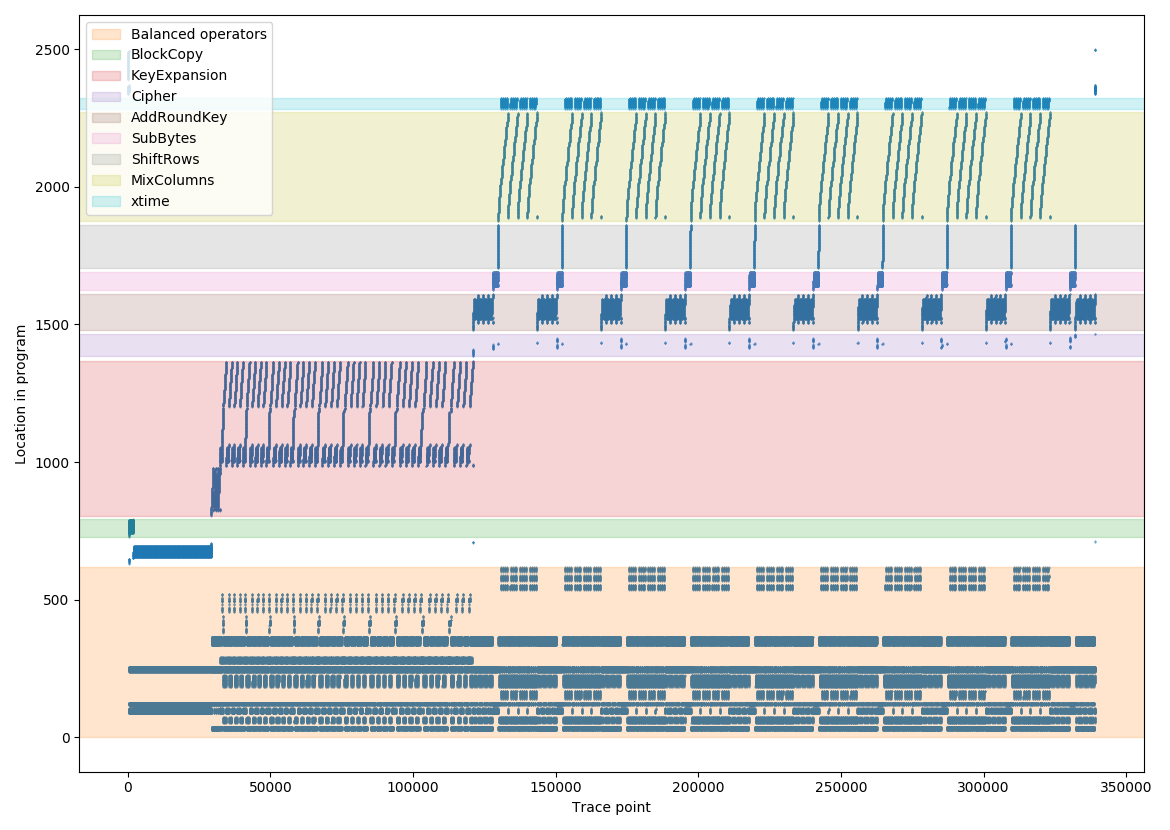
\includegraphics[width=\textwidth]{aes-parts.png}
  \caption{Program regions of AES functions}
  \label{fig:aes}
\end{sidewaysfigure}

\begin{sidewaysfigure}[h]
  \centering
  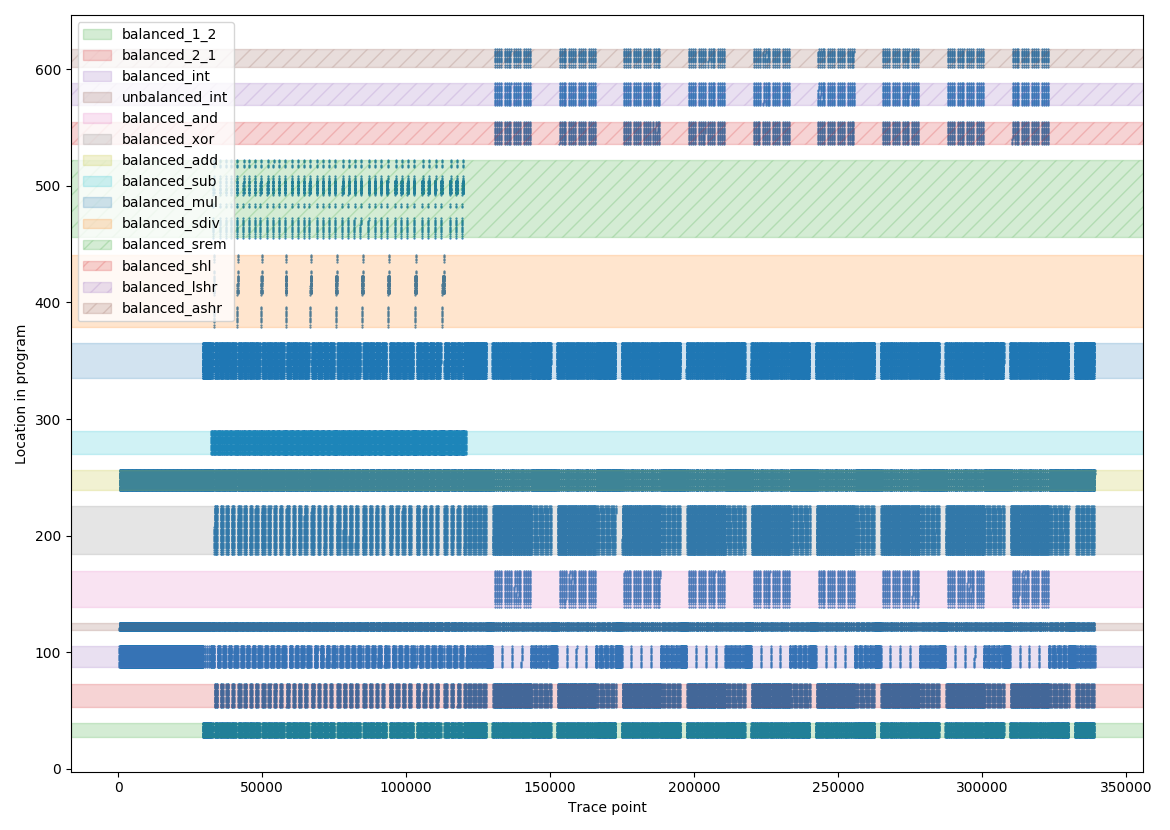
\includegraphics[width=\textwidth]{balanced-ops.png}
  \caption{Program regions of balanced operators}
  \label{fig:ops}
\end{sidewaysfigure}

\begin{sidewaysfigure}[h]
  \centering
  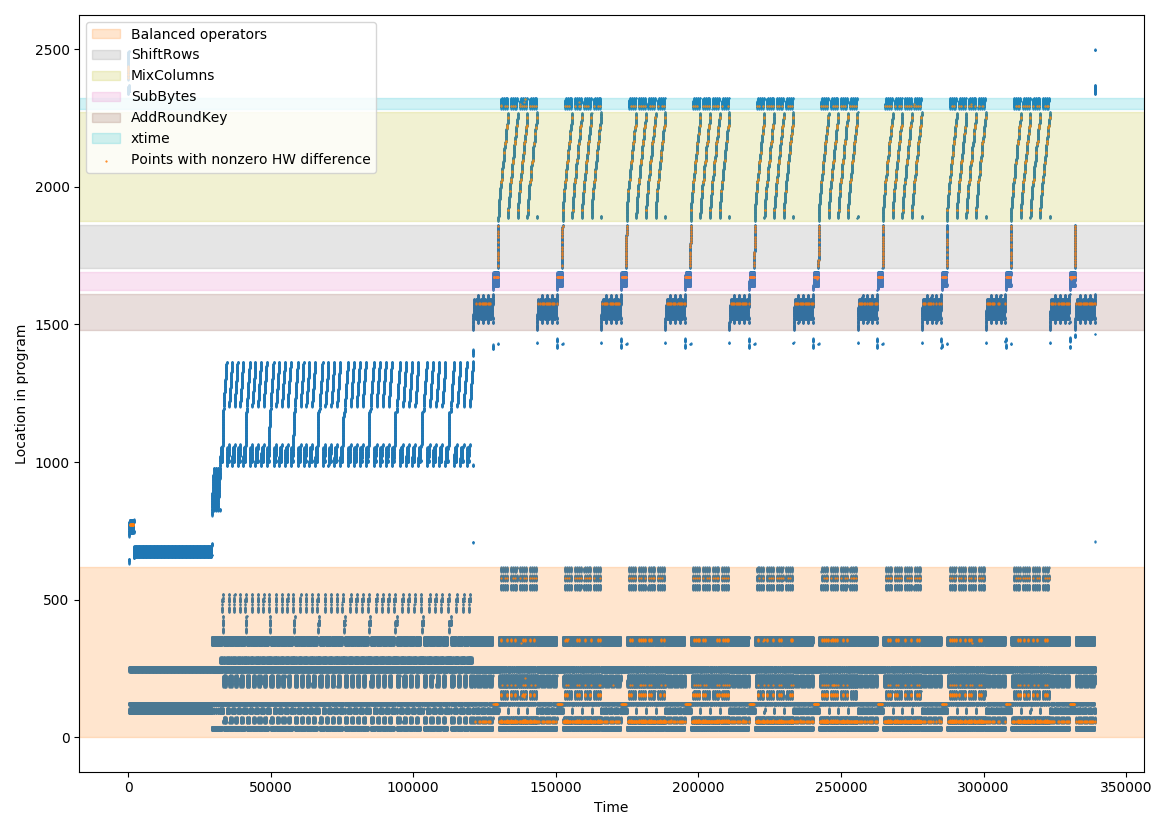
\includegraphics[width=\textwidth]{imbalances-0.png}
  \caption{\hammingw{} differences in power trace}
  \label{fig:imbalances0}
\end{sidewaysfigure}

\begin{sidewaysfigure}[h]
  \centering
  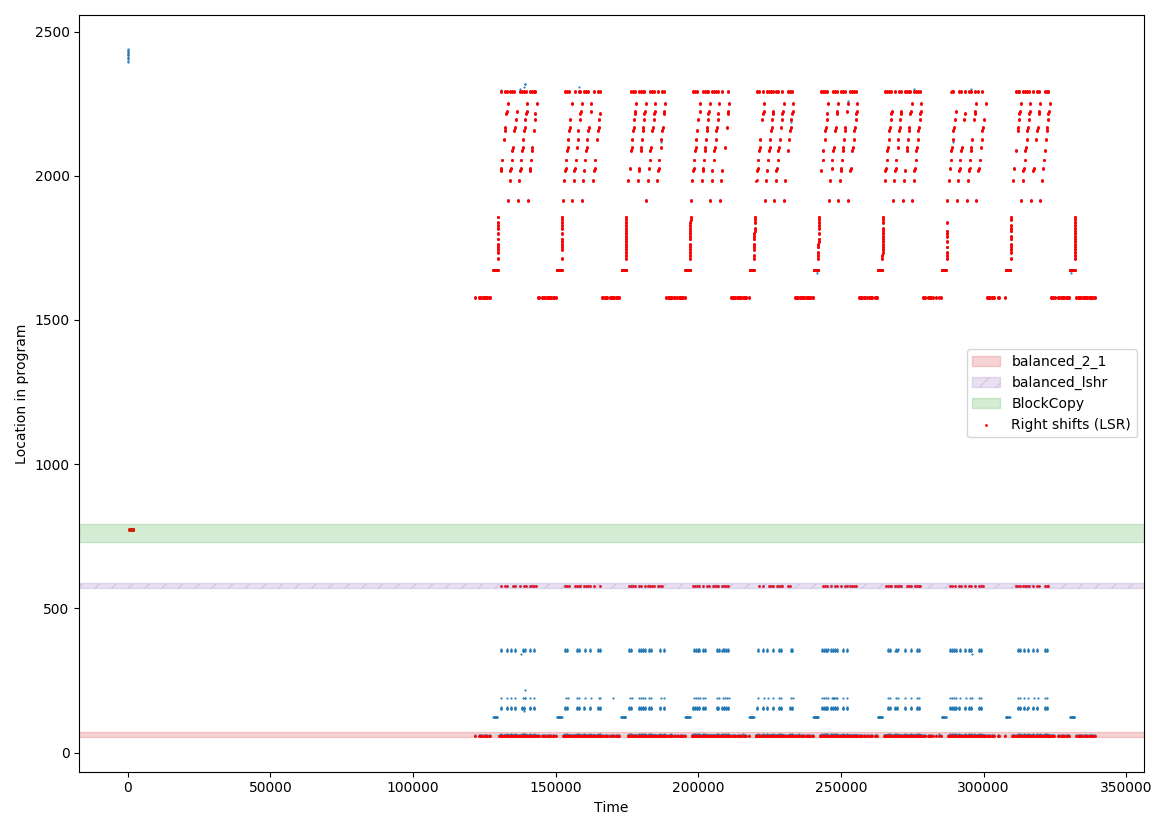
\includegraphics[width=\textwidth]{imbalances-1.png}
  \caption{\hammingw{} differences due to right shifts}
  \label{fig:imbalances1}
\end{sidewaysfigure}

\begin{sidewaysfigure}[h]
  \centering
  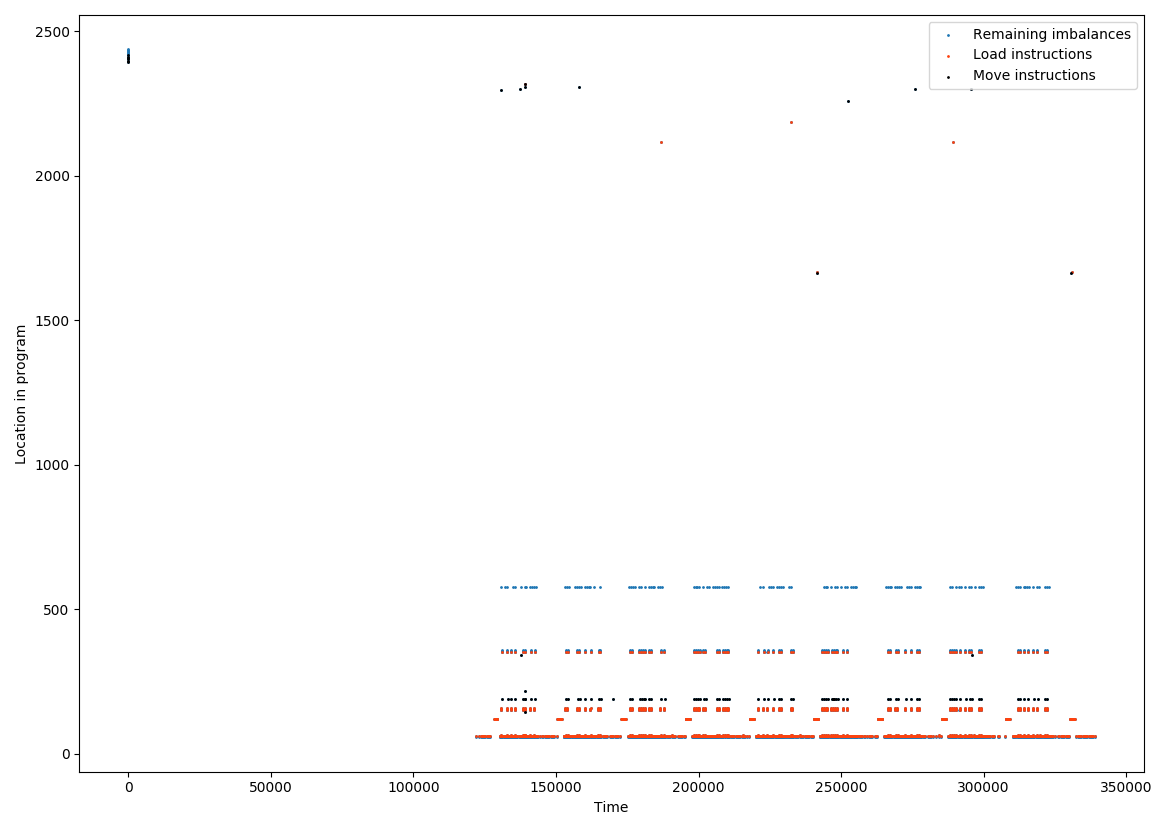
\includegraphics[width=\textwidth]{imbalances-2.png}
  \caption{\hammingw{} differences due to load and move instructions}
  \label{fig:imbalances2}
\end{sidewaysfigure}

\begin{sidewaysfigure}[h]
  \centering
  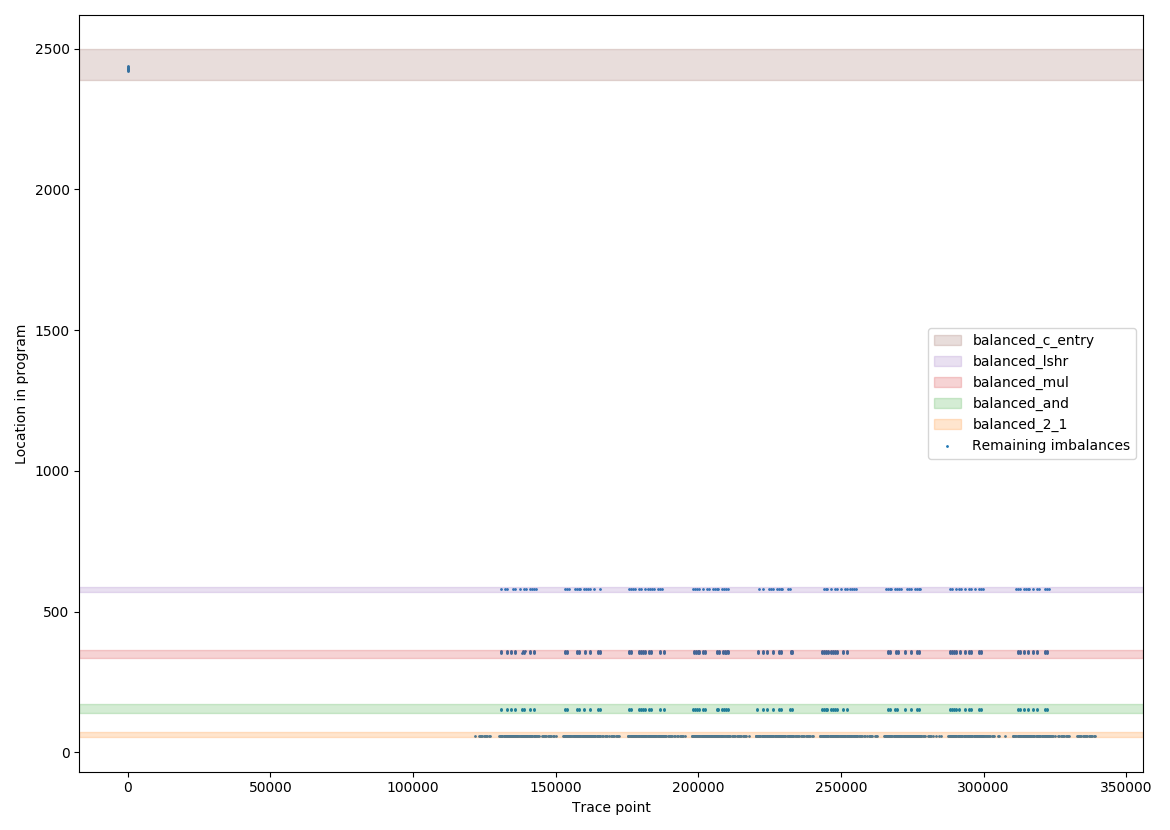
\includegraphics[width=\textwidth]{imbalances-3.png}
  \caption{Sources of imbalanced intermediates}
  \label{fig:imbalances3}
\end{sidewaysfigure}

\section{Performance}
The current balancing pass increases the number of instructions by a factor of 14.888.
This increase is caused by the more complicated balanced operators and overhead for additional function calls.
These additional calls are because currently my operators are implemented as functions, in order to minimize the increase in code size.
More inlining would be possible, which would reduce the number of instructions, but increase the code size.

Additionally, there might be faster variants of implementing the balanced operators.
One could even consider accepting some more information leakage to reduce the number of intermediate operations required.
Taking hardware specifics, such as the ARM barrel shifter into account could also help reduce the performance impact.
Hardware specific optimizations would however reduce the generality of my balancing pass.
The focus of this thesis was to test wether such a balancing pass was \emph{possible}, so performance optimizations are left for future work.
